%%%%%%%%%%%%
\section{General considerations on the Transfer Matrix}
%%%%%%%%%%%%
Let's suppose a 1D system of size $L_X$ where each site can have a height comprised between $-L_Y$ and $L_Y$ with a nearest-neighboors interaction, giving an Hamiltonian $H$ of the form $H = \sum_{i=0}^{L_X} H(i,i+1)$, where the sum is taken over all particles. 
For the following, we will consider an interaction between particles of the form
\begin{align}
  H(i,j) = J f(i,j) + B g(i,j) 
  \label{hamiltonian}
\end{align}
with $f(i,j)$ beeing the interaction between nearest neighboors and $g(i,j) = \frac{g(i)+g(j)}{2}$ a symetrized magnetic field interaction.

We consider the subset of hamiltonians which are symetric with respect to their two variables and periodic boundary conditions along the x-axis.
Summing this hamiltonian over all configurations $\sigma_i$ we get the partition function $Z$ at a temperature $\beta$.
\begin{align*}
 Z &= \sum_{\sigma_1 \sigma_2 ... \sigma_{L_Y}} e^{- \beta H } \\
   &= \sum_{\sigma_1 \sigma_2 ... \sigma_{L_Y}} e^{- \beta \sum_{i} H(i,i+1)}  \\
   &= \sum_{\sigma_1 \sigma_2 ... \sigma_{L_Y}} \prod_{i} e^{-\beta H(i,i+1)} \\
   &= \sum_{\sigma_1 \sigma_2 ... \sigma_{L_Y}} \prod_{i} T(i,i+1)
\end{align*}

Here we introduced a transfer matrix $T(i,j)$ which is symetric. Thanks to the perdiodic boundary conditions of our system, we also have that $T(N,N+1) = T(N,1)$. In that case, the partition function simplifies 
\begin{align}
  Z = Tr T^{L_X}  = \sum_\lambda \langle\lambda | T^{L_X} | \lambda\rangle = \sum_\lambda \lambda^{L_X}
\end{align}
where $|\lambda\rangle$ are the eigenvectors of the partition function with eigenvalues $\lambda$. In the thermodynamic limit where ${L_X}  \rightarrow \infty$ all the eigenvalues will become negligible in comparison to the biggest one $\lambda_0$. 
In this limit, the partition function becomes $Z \simeq \lambda_0^{L_X}$ .

%%%%%%
\subsection{Density probability}
%%%%%%

To compute the probability density of a site to be at a given height, we introduce the orthogonal base of heights $|h\rangle$ where $h_i$ is the height at site $i$, in the definition of our partition function. Using the symetry $\langle\lambda|h\rangle = \langle h|\lambda\rangle$,
\[ 1 = \sum_h \frac{1}{Z} \sum_\lambda \lambda^{L_X} \langle\lambda | h \rangle^2 \]
That allows us to define a density probability $p(h)$ by identification such as 
\begin{align}
  p(h) = \frac{1}{Z} \sum_\lambda \lambda^{L_X} \langle\lambda | h \rangle^2 
  \label{density}
\end{align}

%%%%%%
\subsection{Free energy}
%%%%%%

From the partition function, we define the internal energy of our system as the average of the energy of all our microstates. However, this energy has a dependency with respect to the size of our system. The free energy per site, defined in the thermodynamic limit as 
\begin{align} 
  F &=  - \frac{1}{L_X \beta} \ln(Z) \\
    &\simeq - \frac{1}{\beta } \ln( \lambda_{max})
  \label{deffree_energy}    
\end{align}
measures the difference of energy between two systems of size $L_Y$ and $L_{Y+1}$.

From this, the magnetisation per site is defined as the mean value of the magnetic interaction 
\begin{align}
  m = \langle \sum_{i} g(i,i+1) \rangle = -\frac{\partial F}{\partial B} \Bigr|_{\substack{L}}
\end{align}

Hence, if we wish to compute the free energy of our system for a given length, we can integrate over the magnetic fields. This method is usefull if we do not have access to the eigenvalues of our partition function, as for example in the case of a conserved order dynamics. The free energy is thus given by
\begin{align}
  F(0) - F(B^\ast) = \int_0^{B^\ast} m(B) dB
  \label{free_energy}
\end{align}
Depending on the form of our magnetic interaction, the limit for $B^\ast \rightarrow \infty$ can be derived analytically from the limit state of our system. The integration over the magnetic intensity $B$ can be done numerically using Simpson's rule for an accurate estimate. 

If we have a transfer matrix (in the Glauber dynamics), the magnetisation is directly related to the probability distribution \ref{density} as 
\begin{align}
  \langle m\rangle = \sum_{i=0}^{L_X} p(h_i) h_i = \frac{Tr( D T^{L_X})}{Z}
\end{align}
where $D = \delta_{h h'} h $ is a diagonal matrix representing the possible heights of our sites.
In the limit $L_X$ big, this relation simplifies into 
\begin{align}
  \langle m\rangle = <\lambda_{max}|D|\lambda_{max}>
\end{align}

In numerical simulations we can be interested in the quality of our integral over the magnetisation, simpler said the quality of the magnetisation measurement. The variance of the magnetisation is given by
\begin{align}
  \sigma^2 &= \langle m^2\rangle-\langle m\rangle^2 = \langle (\sum_{i} g(i,i+1))^2 \rangle - \langle \sum_{i} g(i,i+1) \rangle^2 \\
  &= \frac{\partial^2 F}{\partial B^2} \Bigr|_{\substack{L}} - \left( \frac{\partial F}{\partial B} \Bigr|_{\substack{L}} \right) ^2
\end{align}

The second term of the variance has already been computed in the magnetisation. However, the first one is also easy to compute since
\begin{align}
  \frac{\partial^2 F}{\partial B^2} = \frac{\partial m}{\partial B}
\end{align}
In the end, the variance is given by
\begin{align}
  \sigma^2(B^\ast) = \frac{\partial \langle m(B^\ast)\rangle}{\partial B} - \langle m(B^\ast)\rangle^2
\end{align}
A Q factor can be introduced to have the numerical noise for a given hamiltonian, be it from direct diagonalization of the transfer matrix or from numerical integration defined by
\[ Q(B) = \frac{\langle m(B)\rangle}{\sigma(B)} \]
The bigger the Q the better is our signal-to-noise ratio. This measurement would be a good indicator of \textcolor{red}{still don't really get how we can use this later}
 
%%%%%%%%%%%%
\newpage
\section{SOS Hamiltonian}
%%%%%%%%%%%%

In the following, we present three Solid-On-Solid models with different magnetic fields. 
The SOS interaction between nearest neighboors is of the form $f(i,j) = |h_i - h_j|$. 
This kind of interaction prevents big fluctuations between two nearest neighboors and is directly related to the Ising model in the approximation where there are no overhangs between the two phases. \textcolor{blue}{see my notes for the derivation}

In the absence of a magnetic field, the interface will fluctuate around its center. Shown below an typical SOS interface for an $L_X=50$ and a $L_Y=60$ after $10^5$ Monte Carlo steps.

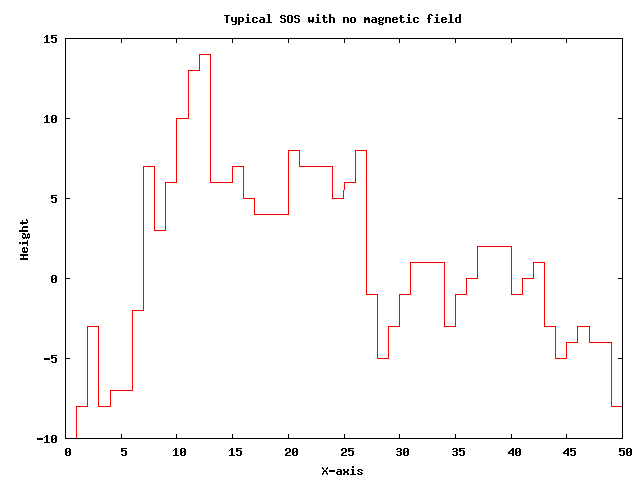
\includegraphics{tm/nomag.png}


%%%%%%
\subsection{Model $g(i) = h_i$ (model A)}
%%%%%%

This model replicates the effect of a homogeneous magnetic field. The bigger the magnetic field $B$ (which can be positive or negative), the further the interface is driven with a symetry breaking. 

\begin{align}
  H(i,j) = J |h_i-h_j| + B \frac{h_i + h_j}{2}
\end{align}

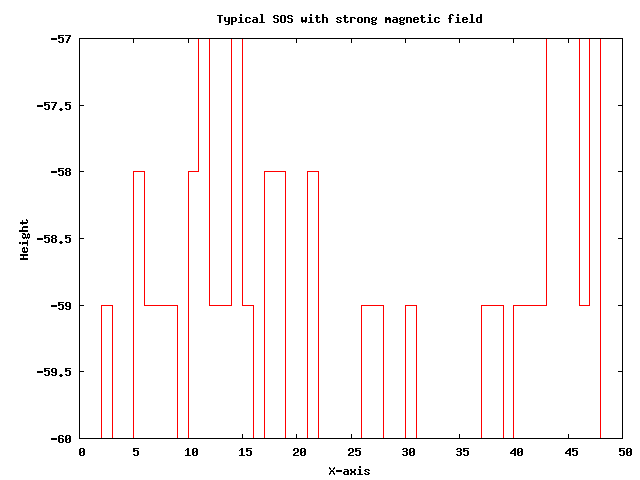
\includegraphics{tm/normal.png}

For an infinite magnetic field, we clearly see that the interface gets flattened over on of the edge. The resulting single state avalaible in this limit is the flat interface, with all sites beeing over or under it, depending on the sign of $B$.

In the limit $B \rightarrow \infty$, the interface will flatten to the bottom edge, resulting in a single state of energy 
\begin{align}
  F(B \rightarrow \infty) = - B L_Y
\end{align}

The free energy for at $B=0$ is thus given by equation \ref{free_energy} as
\begin{align}
  F(0) = B L_X L_Y - \int_0^\infty m(B)dB
  \label{energymodela}
\end{align}
with $m(B) = \langle\sum_i h_i\rangle = L_Y$

%%%%%%
\subsection{Model $g(i) = |h_i|$ (model B)}
%%%%%%

This model uses a stagged magnetic field analoguous to the action of a laser on a binary mixture. The further we get from the mean position, the higher is the energy. In order to minimize the energy, the system will have a tendency to be pinned, leading to a very flat interface. 

\begin{align}
  H(i,j) = J |h_i-h_j| + B \frac{|h_i| + |h_j|}{2}
\end{align}

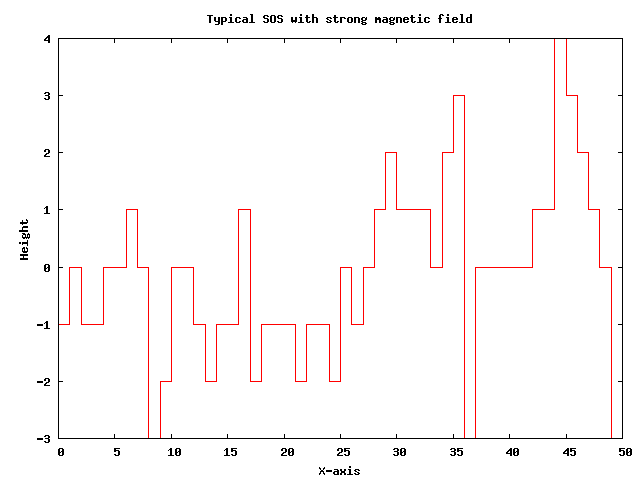
\includegraphics{tm/stagged.png}

In the limit $B \rightarrow \infty$, the free energy $F$ will be equal to $0$, while the magnetisation $m(B \rightarrow \infty) = \langle\sum_i |h_i|\rangle = 0$ also.

%%%%%%
\subsection{Model $g(i) = -|h_i|$ (model C)}
%%%%%%

This model is the same as the previous one, except with a switch of sign. In this case, the magnetic field will have a depinning effect leading to a scattering of the heights around both edges. \textcolor{red}{I don't really get yet the argument about the competition between entropy and energy.}

\begin{align}
  H(i,j) = J |h_i-h_j| - B \frac{|h_i| + |h_j|}{2}
\end{align}

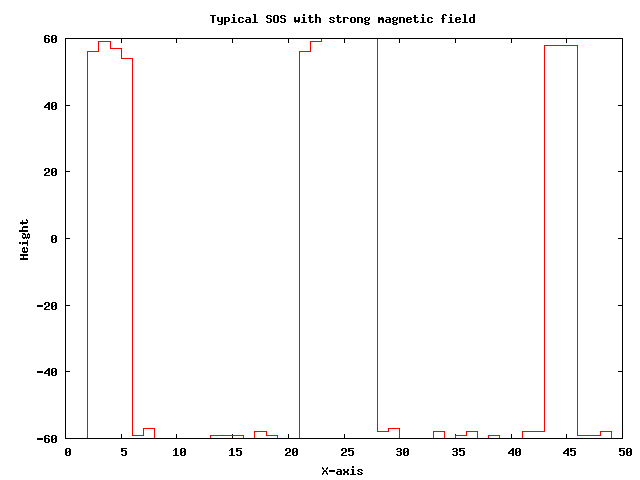
\includegraphics{tm/negstagged.png}

In the $B \rightarrow \infty$ limit, we have then a scattered system. How can we compute its free energy ? Sites will be at $h_i=\pm L_Y$ , leading to an easy $2\times 2$ transfer matrix.
\begin{align}
  Z = e^{\beta B L_Y L_X} Tr( (e^{-\beta J \frac{L_Y}{2} \sum_i |\sigma_i - \sigma_j| })^{L_X} )
\end{align}
where $\sigma_i = \pm 1$

The transfer matrix is then given as

\begin{align}
T= e^{\beta B L_Y}
  \begin{pmatrix}
    1 & e^{-\beta 2 J L_Y} \\
    e^{-\beta 2 J L_Y} & 1
  \end{pmatrix}
\end{align}
Its eigenvalues are $\lambda_\pm = e^{\beta B L_Y}( 1 \pm e^{-\beta 2 J L_Y})$, giving a partion function 
\begin{align}
  Z = e^{\beta B L_Y L_X} \times ((1 - e^{-\beta 2 J L_Y})^{L_X} + (1 + e^{-\beta 2 J L_Y})^{L_X} )
\end{align}

The free energy from \ref{deffree_energy} is 
\begin{align}
  F(B\rightarrow \infty) = - L_Y B - \frac{1}{\beta} \ln \left( 1 + e^{-\beta 2 J L_Y} \right)
  \label{energymodelc}
\end{align}
which, in the limit of $L_X \rightarrow \infty$ converges to \ref{energymodela}. This is easily explained as the energy to switch from a side to another increases so much that at some point the interface will be pinned to one of the edges, resulting in the same single state.

\begin{figure}
  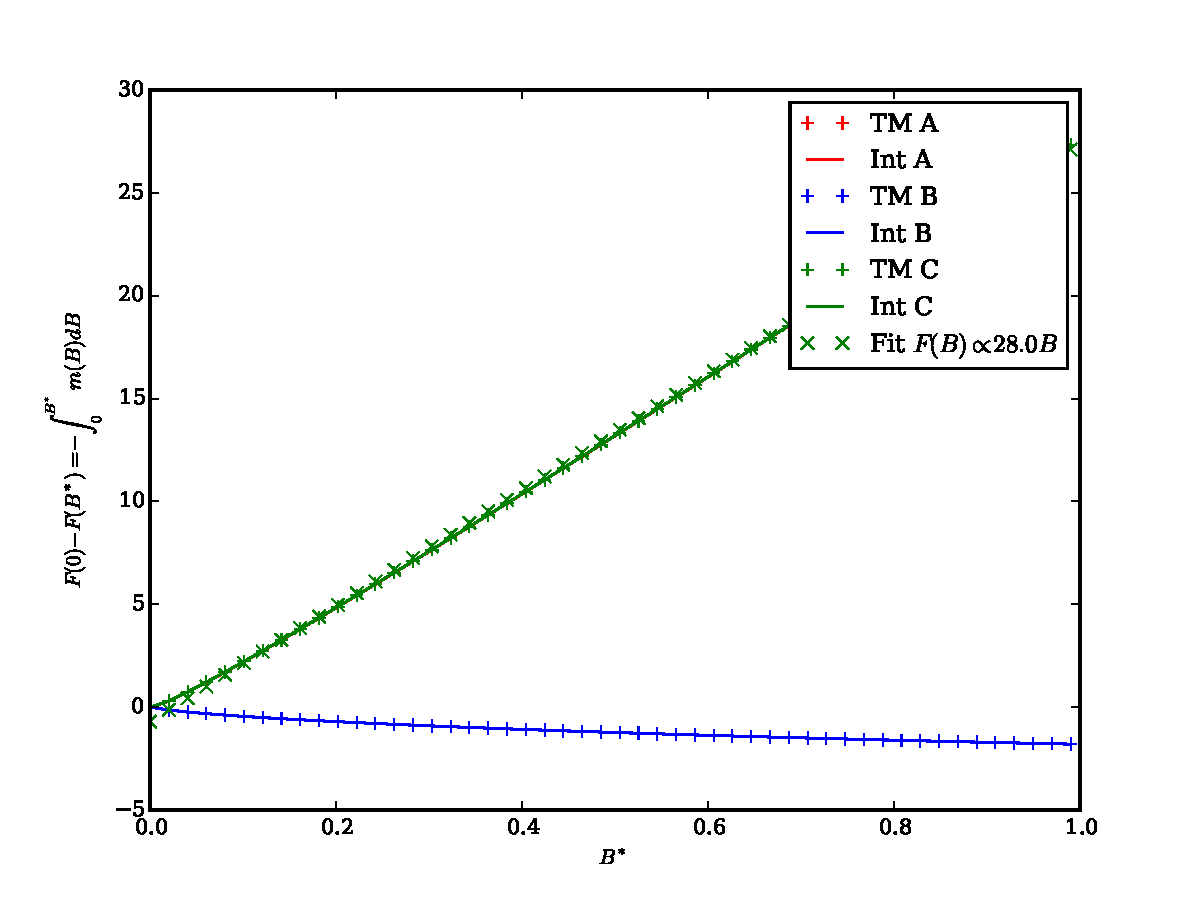
\includegraphics[width=13cm]{tm/comparison.pdf}
  \caption{Computation of both terms in \ref{free_energy} in the limit $L_X \rightarrow \infty$ and $L_Y=30$ for the three different models. We see that models A and C have a very similar behaviour even for very small $B$. The linear fit does indeed give a relation $F(0) - F(B) = L_Y \times B$}
\end{figure}

%%%%%%%%%%%%
\newpage
\section{Numerical results}
%%%%%%%%%%%%

The diffusion of particles in a system can be mapped in an Ising model pretty easily if we assume the conservation of particles through time in our Monte Carlo dynamics. That means that $\sum h_i = K$, with $K$ a constant defined by the initial conditions. This condition can be enforced in the partition function if we only take the microstates satisfying our constraint. Sadly, this constraint is about the microstates and can not be transposed into our Hamiltonian, making the Transfer Matrix useless for such a case. 

The question we want to adress is thus : how big is the difference between the constrained and the unconstrained dynamic in the computation of the free energy ? Is the limit $B^{\ast} \rightarrow \infty$ the same for the three models for both dynamics ? 
Figure \ref{compGlau} conforts us in the conformity between the Glauber dynamic and the Transfer Matrix method. 

\begin{figure}[h]
  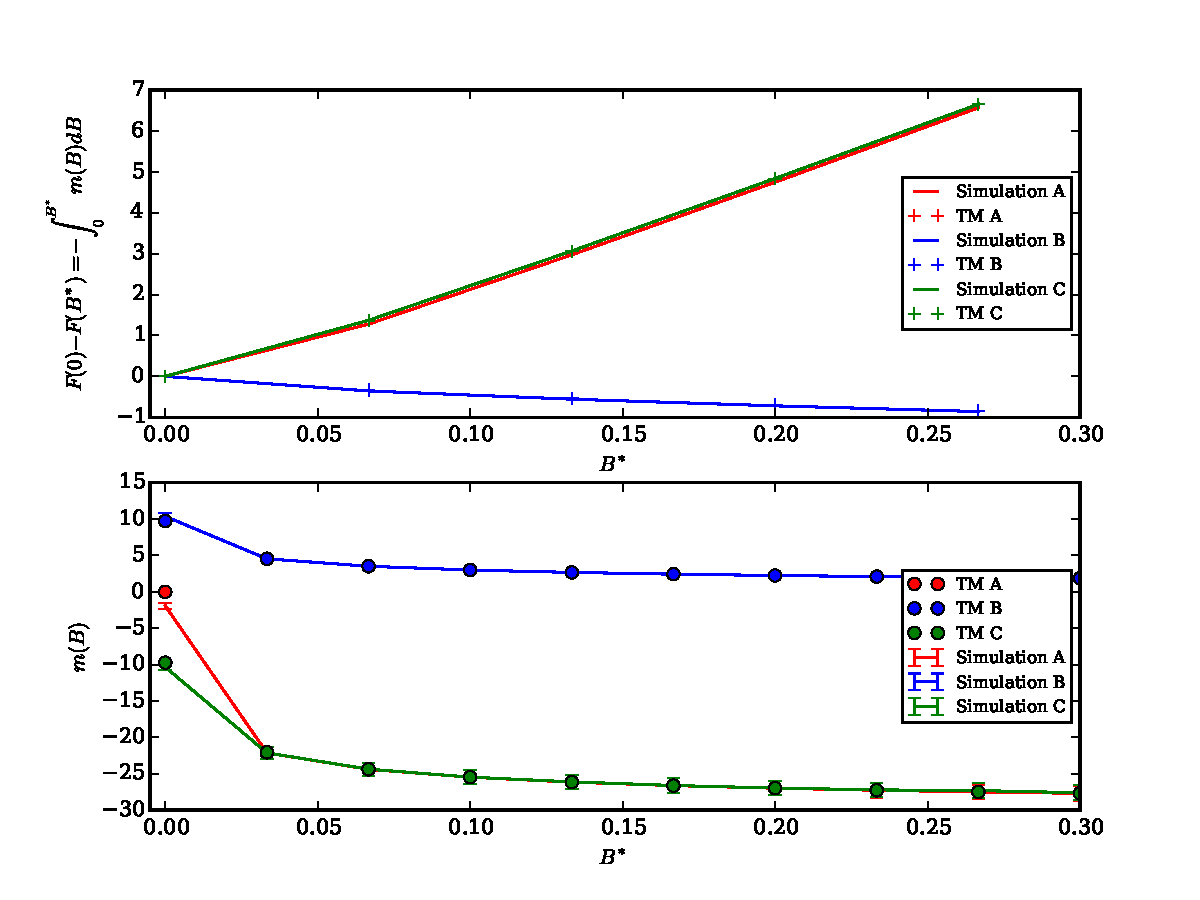
\includegraphics[width=13cm]{tm/ModGlau.pdf}
  \caption{Computation of the free energy (above) and the magnetisation (below) for the three models in a Glauber dynamics (unconstrained dynamics) through simulations (with error bars) and exact transfer matrix diagonalization.}
  \label{compGlau}
\end{figure}

When comparing to the Kawasaki dynamic in Figure \ref{compKaw}, we start seeing some differences. First, in model A the magnetization of our system is always  equal to $0$, by construction of our Kawasaki dynamics, meaning that the computation of the free energy is a tricky one. Luckily, Model A is very similar to Model C with respect to the posible microstates, except some walls that do not add a significan free energy into the system. This means that the results we obtain in Model C are roughly the same as in Model A ! This allows us to drop Model A from the discussion from now on and get retrieve its general behaviour and properties from Model C.

As expected, the constrained dynamics adds some variance with respect to the Transfer Matrix. 

\begin{figure}
  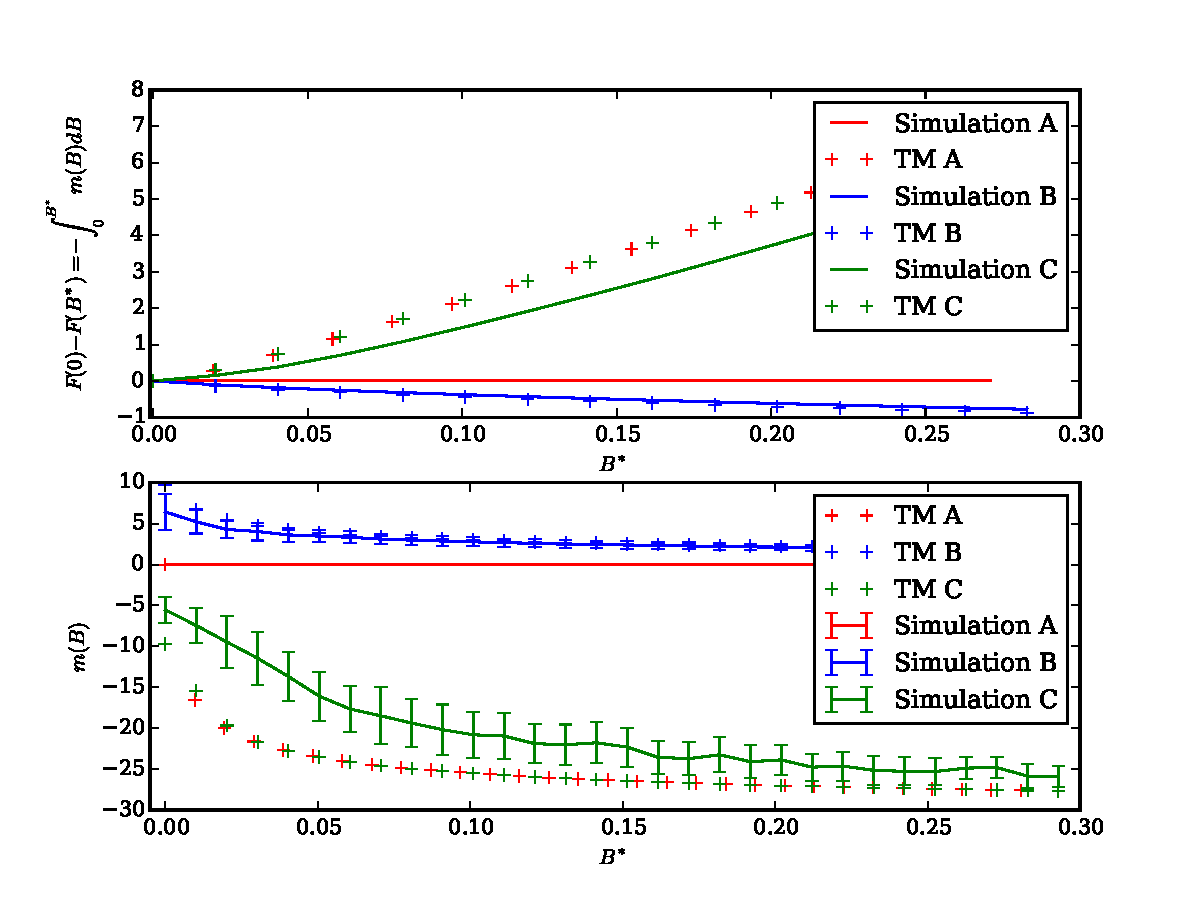
\includegraphics[width=13cm]{tm/ModKaw.pdf}
  \caption{Computation of the free energy (above) and the magnetisation (below) for the three models in a Kawasaki dynamics (constrained dynamics) through simulations (with error bars) and exact transfer matrix diagonalization. The error in magnetization of Model A is exactly equal to 0, by construction.}
  \label{compKaw}  
\end{figure}
